\documentclass [bachelor,ngerman,a4paper,11pt,oneside,webreferences,glossary,indextop,listoflistings,listofalgorithms,acronyms]{INSOthesis}
% change encoding in the document
%\inputencoding{utf8} % default
%\inputencoding{latin1} % for windows

\thesistitle{Durchführung einer Relay Attacke durch Interception der Android NFC-Schnittstelle}
%\thesisshorttitle{Shorttitle of the Thesis}
%\thesissubtitle{Optional Subtitle} % optional
\thesisdate{\today}

% all titles and designations have to be gender-related!
%\thesistype{Diplomarbeit}{Master's Thesis}
%\thesisdegree{Diplom-Ingenieurin}{Diplom-Ingenieurin}
\thesiscurriculum{Software \& Information Engineering}{Software \& Information Engineering} % your study
\thesisauthor{Michael Peyerl} % your name
\thesisauthoraddress{Hagsdorf 26, 3680 Persenbeug} % your address
\thesismatrikelno{1326027} % your registration number

% advisor
%\thesisauthorpreamble {Verfasser}
%\thesisadvisorpreamble {Betreuung}
%\thesisadvisorone {Thomas Grechenig}
\thesisadvisortwo {Clemens Hlauschek}
%\thesisadvisorthree {Vorname Nachname}

% Bibliographie file
\bibliography{bibliography/references}

\hypersetup{
  %colorlinks=false % enable and disable frames arround links
}

%%%%%%%%%%%%%%%%%%%%%%%%%%%%%%%%%%%%%%%%%%%%%
%
% Can be used to add additional informations
%
%%%%%%%%%%%%%%%%%%%%%%%%%%%%%%%%%%%%%%%%%%%%%
% \AfterTitlePages{}
% \AfterDeclaration{}
% \AfterAcknowledgements{}
% \AfterAbstract{}
% \AfterListOfFigures{}
% \AfterListOfTables{}
% \AfterAbbreviations{}
% \AfterBibliography{}

\renewcommand\afterchapternum{\hspace{1em}}
\begin{document}

\maketitle

%%%%%%%%%%%%%%%%%%%%%%%%%%%%%%%%%%%%%%%%%
%%%   CONTENTS    %%%%%%%%%%%%%%%%%%%%%%%
%%%%%%%%%%%%%%%%%%%%%%%%%%%%%%%%%%%%%%%%%

%%%%%%%%%%%%%%%%%%%%%%%%%%%%%%%%%%%%%%%%%%%%%%%%%%%%%%%%%%%%%%%%%%%%%%%%
\chapter{Einleitung}
\label{sec:introduction}
%%%%%%%%%%%%%%%%%%%%%%%%%%%%%%%%%%%%%%%%%%%%%%%%%%%%%%%%%%%%%%%%%%%%%%%%

In der Einleitung soll die Zielsetzung der Arbeit beschrieben, ihre Einordnung in einen übergeordneten Kontext hergestellt und die Bedeutung des Themas erörtert werden. Zu diesem Zweck ist die Einleitung in folgende Unterkapitel unterteilt:
\begin{itemize}
	\item Problemstellung
	\item Motivation
	\item Zielsetzung
	\item Aufbau der Arbeit
\end{itemize}

\makeatletter
\ifthesis@masterthesis
Durch die Einleitung sollen folgende Punkte in den jeweiligen Unterkapiteln klargestellt werden:
\begin{itemize}
	\item Etwaige thematische Einschränkungen bzw. Auswahl und Begründung der Bearbeitungsziele
	\item Betrachtung verschiedener methodischer Alternativen zur Aufgabenlösung und Erklärung der Entscheidung
	\item Gewählter Lösungsansatz, z.B. theoretische Untersuchung, Literaturauswertung und -vergleich oder eine empirische, auf eigenen Erhebungen basierende Untersuchung
\end{itemize}
\fi
\makeatother

\paragraph{Organisatorisches}
\makeatletter\ifthesis@masterthesis
Bitte einen Zeitplan für die Verfassung Ihrer Diplomarbeit erarbeiten und mit Ihrem Betreuer abstimmen. Es gibt sehr \enquote{kurzlebige} Themenstellungen, die rasch an Aktualität verlieren, da ist der Zeitplan unbedingt einzuhalten, ansonsten wird das Thema neu vergeben. Bei Themen, die länger aktuell bleiben, kann der Zeitrahmen auch länger erstreckt werden, dies aber bitte im Vorfeld abklären! Üblicherweise sollte die Verfassung einer Diplomarbeit ein halbes Jahr bis ein Jahr dauern, Ausnahmen bitte zumindest durch regelmäßigen email-Kontakt abstimmen.
\fi\makeatother

Der Umfang einer Diplomarbeit beträgt üblicherweise 90 bis ca. 120 Seiten und bei Bachelorarbeiten 40 bis ca. 60 Seiten. Beurteilungskriterien für eine Diplomarbeit ist nicht nur die Qualität der praktischen Arbeit, sondern auch Aufbau, Inhalt und Formulierung der schriftlichen Arbeit. Insbesondere sind die Grundregeln wissenschaftlichen Arbeitens (z.B. richtiges Zitieren) zu beachten.

\paragraph{Allgemeines}
Achtung beim Setzen von Absätze.

Fußzeilen: Bei technischen Arbeiten eher unüblich. \\
In den Sozialwissenschaften (z.B. BWL) ist es üblich, die Referenz in eine Fußnote zu setzen.
\\
In den technischen Wissenschaften ist es üblich, im Text ein Kürzel (Dorn et al. 1999) oder eine Zahl [1] zu verwenden, um dann im Anhang der Arbeit alle Referenzen detailliert aufzuführen, wobei jede Referenz mit dem Kürzel beginnt.

Bei einer wissenschaftlichen Arbeit wird Wert auf die Einhaltung formaler Aspekte des guten Schreibens gelegt. Es ist hilfreich, wenn man seinen eigenen Schreibstil kritisch in Bezug auf folgende Punkte überprüft:
\begin{itemize}
	\item Einfachheit (das \ac{KISS}-Prinzip gilt nicht nur für die Softwareentwicklung, sondern auch für wissenschaftliche Arbeiten: Mach es schlicht und wesentlich/\acl{KISS})
	\item Gliederung/ logische Ordnung (vom Allgemeinen zum Konkreten, nachvollziehbare Kette von einer Fragestellung/ einem Problem über die Bearbeitung und Zerlegung in Detailprobleme zur Lösung und der Ableitung von Erkenntnissen)
	\item Kürze/Prägnanz (keine Schachtelsätz, Wiederholungen vermeiden – \enquote{Don't repeat yourself})
	\item Anregende Zusätze (erläuternde/ interessante/ spannende Praxisbeispiele etc.)
	\item Sprache/Stil (kein Erzählstil, möglichst keine \enquote{ich}-Form, objektiv)
	\item Korrekte Formeln und Abbildungen
	\item Korrekte Zitierweise (siehe Kapitel Literaturverzeichnis)
	\item Einhaltung definierter Rahmenbedingungen (z.B. diese Vorlage)
	\item Vermeiden von Anglizismen. Grundsätzlich sollte in einer in Deutsch verfassten Diplomarbeit immer das deutsche Wort verwendet werden, wenn es unmissverständlich und akzeptiert ist. Ein Eindeutschen um jeden Preis ist allerdings zu vermeiden, da dies zu schwer lesbaren Texten führt. Beispiele: Der Begriff \enquote{Unterbrechung des Programmflusses} ist angebrachter als \enquote{Interrupt des Programmflusses}, und \enquote{verdeckte Kanäle} ist als akzeptierter deutscher Begriff für \enquote{Covert Channels} zu verwenden. Umgekehrt ist aber \enquote{Cursor} das bessere Wort als \enquote{Lichtmarke}. Anglizismen können als Stilmittel genutzt werden, etwa wenn man von einer \enquote{Quick and Dirty} Implementierung spricht.
\end{itemize}

\paragraph{Typographie}
Grundsätzlich sollten nicht mehr als drei unterschiedliche Schriftarten verwendet werden. Grundsätzlich sollte die Typographie sowie die Anordnung von Bildern, Tabellen, etc. \LaTeX überlassen werden. Allerdings können Silbentrennungen durch \verb|\-| gesteuert werden.

Abweichungen nach persönlichem Geschmack und in Rücksprache mit Ihrem Betreuer sind zulässig. Als Stilmittel werden üblicherweise nur die Fettschrift und Kursivschrift verwendet - Unterstreichungen, Schattenschriften etc. sind zu vermeiden. Blocksatz bitte mit automatischer Silbentrennung verwenden, Rechtschreibprüfung aktivieren.

Generell kann bei der Einleitung eine modifizierte Version des Exposés als Basis verwendet werden.

%=======================================================================
\section{Problemstellung}
%=======================================================================

Formulierung der Problemstellung, Einbettung in das Forschungsumfeld und Theorie, auf die sich die Arbeit beziehen. Tendenziell kurz, allgemeiner und sehr gut verständlich -- detaillierter im Kapitel \enquote{Grundlagen}.

Die formulierte Fragestellung soll das Interesse an der Lösung wecken (eine langweilige oder triviale Problemstellung lässt meistens auch eine eher weniger interessante wissenschaftliche Arbeit erwarten).

\makeatletter\ifthesis@masterthesis
Nach dem Lesen dieses Kapitels sollten folgende Punkte klar dargestellt sein:
\begin{itemize}
	\item Welche konkrete Fragestellung/Arbeitshypothese/welches Problem liegt dem Thema zugrunde?
	\item Klare Definition des Untersuchungsgegenstands (z.B. effiziente Internationalisierung/ Mehrsprachigkeit von Computerprogrammen im Java Umfeld).
	\item Darlegung und Begründung thematischer Abgrenzungen.
	\item Klare Darstellung eines ggf. übergeordneten fachlichen Kontexts/Zusammenhangs (z.B. des medizinisch/ organisatorischen Rahmens, der bei einer Arbeit über Usability einen Einfluss auf die Usability einer auf Tablets/Touchscreens basieren Pflegedokumentation im klinischen Bereich hat).
\end{itemize}

In diesem Kapitel wird das Problem und sein Kontext beschrieben (\enquote{die Sache/die Frage}) – nicht aber, warum es gerade zum Zeitpunkt der Diplomarbeit notwendig ist, für dieses Problem eine Lösung zu erarbeiten. Das \enquote{Warum} (die Motivation) wird im nächsten Unterkapitel beschrieben.
\fi\makeatother

%=======================================================================
\section{Motivation}
%=======================================================================

In diesem Kapitel wird der Forschungsbedarf aufgezeigt. Nach dem Lesen dieses Kapitels sollten folgende Punkte klar dargestellt sein:
\begin{itemize}
	\item Aktueller Stand der Wissenschaft in Bezug auf die zuvor formulierte Problemstellung und klare Darstellung, was hier unzureichend/offen ist.
	\item GGf. Darstellung des größeren Forschungsbereichs, in den die Diplomarbeit eingebettet ist.
	\item Darlegung der Bedeutung des Themas für den Stand oder die Weiterentwicklung eines Bereichs der Informatik (z.B. Datenbanksysteme, Mobile Anwendungen, Java-Programmierung, Rechenzentrumsbetrieb, \dots) oder eines Fachbereichs (z.B. Bankwesen, Wertpapierhandel, Gesundheitswesen, Transportwesen, Flugsicherheit \dots). Erklärung, was durch die Lösung des Problems z.B. kostengünstiger/schneller/hochwertiger/sicherer/anwendbarer/\enquote{schöner} etc. wird.
\end{itemize}

%=======================================================================
\section{Zielsetzung}
%=======================================================================

Nachdem die Problemstellung und die Motivation zu deren Lösung formuliert wurden, wird in diesem Kapitel das zu erarbeitende Resultat beschrieben.

\makeatletter\ifthesis@masterthesis
Nach dem Lesen dieses Kapitels sollten folgende Punkte klar dargestellt sein:
\begin{itemize}
	\item Umfang, in dem die Problemstellung am Ende der Arbeit gelöst sein soll bzw. mit welchen Einschränkungen.
	\item Methode zur Erarbeitung des Resultats.
	\item Gibt es einen Theorie- und einen Praxisteil?
	\item Schwerpunkte des Praxisteils (z.B. Durchführung einer Umfrage, Programmierung, Herstellung von Hardware, Erprobung einer Methode in einem konkreten Projekt)?
	\item Art des Resultats (z.B. ein Programm, eine Formel, eine Methode, die Erweiterung einer existierenden Methode, ein Konzept, ein Framework, Hardware-Prototyp, eine bewiesene Erkenntnis)?
\end{itemize}
\fi\makeatother

\makeatletter\ifthesis@masterthesis
%=======================================================================
\section{Aufbau der Arbeit}
%=======================================================================

Beispielhaft:

Kapitel \ref{sec:fundamentals} behandelt sowohl Grundlagen als auch Definitionen und bietet einen Überblick \dots, die als Basis für \dots dienen.

\dots, wird in Kapitel 3 erläutert..

Ein Anwendungsszenario (Fallbeispiel), das \dots, ist in Kapitel 4 dargestellt. Dieses Szenario umfasst \dots.

Kapitel 5 setzt sich \dots. auseinander.

Einsatzmöglichkeiten in der Praxis werden in Kapitel 6 diskutiert.

Abschließend fasst Kapitel \ref{sec:conclusion} die wesentlichen Erkenntnisse zusammen und gibt einen Ausblick in die Zukunft.
\fi\makeatother

%%%%%%%%%%%%%%%%%%%%%%%%%%%%%%%%%%%%%%%%%%%%%%%%%%%%%%%%%%%%%%%%%%%%%%%%%%%%%%%%%%%%%%%%%%%%%%%%%%%%%%%%%%%%%%%%%%%%%%%%%%%%%%%%%%%%%%%%%%%%%%%%%%%%%%%%%%%%%%%%%%%%%%%%%%
% \section{General Information}
%
% This document is intended as a template and guideline and should support the author in the course of doing the master's thesis.
% Assessment criteria comprise the quality of the theoretical and/or practical work as well as structure, content and wording of the written master's thesis. Careful attention should be given to the basics of scientific work (e.g., correct citation).\footnote{Sample Footnote}
%
% \section{Organizational Issues}
%
% A master's thesis at the Faculty of Informatics has to be finished within six months. During this period regular meetings between the advisor(s) and the author have to take place.
% In addition, the following milestones have to be fulfilled:
% \begin{enumerate}
%   \item  Within one month after having fixed the topic of the thesis the master's thesis proposal has to be prepared and must be accepted by the advisor(s). The master's thesis proposal must follow the respective template of the dean of academic affairs. Thereafter the proposal has to be applied for at the deanery. The necessary forms may be found on the web site of the Faculty of Informatics. \url{http://www.informatik.tuwien.ac.at/dekanat/formulare.html}
%   \item  Accompanied with the master's thesis proposal, the structure of the thesis in terms of a table of contents has to be provided.
%   \item Then, the first talk has to be given at the so-called ``Seminar for Master Students''. The slides have to be discussed with the advisor(s) one week in advance. Attendance of the ``Seminar for Master Students'' is compulsory and offers the opportunity to discuss arising problems among other master students.
%   \item At the latest five months after the beginning, a provisional final version of the thesis has to be handed over to the advisor(s).
%   \item As soon as the provisional final version exists, a first poster draft has to be made. The making of a poster is a compulsory part of the ``Seminar for Master Students'' for all master studies at the Faculty of Informatics. Drafts and design guidelines can be found at \url{http://www.informatik.tuwien.ac.at/studium/richtlinien}.
%   \item After having consulted the advisor(s) the second talk has to be held at the ``Seminar for Master Students''.
%   \item At the latest six months after the beginning, the corrected version of the master's thesis and the poster have to be handed over to the advisor(s).
%   \item After completion the master's thesis has to be presented at the ``epilog''. For detailed information on the epilog see: \\ \url{http://www.informatik.tuwien.ac.at/studium/epilog}
% \end{enumerate}
%
% \section{Structure of the Master's Thesis}
%
% If the curriculum regulates the language of the master's thesis to be English (like for ``Business Informatics''), the thesis has to be written in English. Otherwise, the master's thesis may be written in English or in German. The structure of the thesis is predetermined.
% The table of contents is followed by the introduction and the main part, which can vary according to the content. The master's thesis ends with the bibliography (compulsory) and the appendix (optional).
%
% \begin{itemize}
%   \item	Cover page
%   \item Acknowledgements
%   \item Abstract of the thesis in English and German
%   \item Table of contents
%   \item Introduction
%   	\begin{itemize}
%   		\item motivation
%   		\item problem statement (which problem should be solved?)
%   		\item aim of the work
%   		\item methodological approach
%   		\item structure of the work
%   	\end{itemize}
%   \item State of the art / analysis of existing approaches
%   	\begin{itemize}
%   		\item literature studies
%   		\item analysis
%   		\item comparison and summary of existing approaches
%   	\end{itemize}
%   \item Methodology
%   	\begin{itemize}
%   		\item used concepts
%   		\item methods and/or models
%   		\item languages
%   		\item design methods
%   		\item data models
%   		\item analysis methods
%   		\item formalisms
%   	\end{itemize}
%   \item Suggested solution/implementation
%   \item Critical reflection
%   	\begin{itemize}
%   		\item comparison with related work
%   		\item discussion of open issues
%   	\end{itemize}
%   \item Summary and future work
%   \item Appendix: source code, data models, \dots
%   \item Bibliography
% \end{itemize}
%

%%%%%%%%%%%%%%%%%%%%%%%%%%%%%%%%%%%%%%%%%%%%%%%%%%%%%%%%%%%%%%%%%%%%%%%%
\chapter{Grundlagen und Hintergründe}
\label{sec:fundamentals}
%%%%%%%%%%%%%%%%%%%%%%%%%%%%%%%%%%%%%%%%%%%%%%%%%%%%%%%%%%%%%%%%%%%%%%%%

Dieses Kapitel beschreibt Grundlagen und Konzepte, die eine wichtige Rolle als Fundament für das Verständnis der Arbeit einnehmen. In erster Linie wird die Kommunikationstechnologie Near Field Communication (NFC) und ihre Funktionsweise vorgestellt. Es soll behandelt werden, wie NFC technisch umgesetzt ist und mithilfe welcher Komponenten und Methoden die drahtlose Kommunikation erfolgt. Außerdem soll auf die Ausführung der Technologie auf mobilen Android Geräten eingegangen und Sicherheitsrisiken und -konzepte beschrieben werden. Ein äußerst relevanter Punkt im Zusammenhang mit dieser Arbeit ist die Relay Attacke. Das Prinzip hinter diesem Angriff und dessen praktische Ausführung werden ebenfalls behandelt. 

Im Zuge der praktischen Implementierung der Relay Attacke wird mit dem Android Betriebssystem gearbeitet. Dabei werden neben der Entwicklung von Android Applikationen auch Eingriffe in den Android Quellcode selbst notwendig sein. Um die praktische Implementierung der Relay Attacke zu verstehen, ist daher ein grundlegendes Verständnis der Android Architektur sowie der Komponenten zur Entwicklung einer Android Applikation essentiell. Im nachfolgenden Kapitel wird daher vor der Diskussion der mit der NFC Technologie verwandten Themen eine Erläuterung der Grundlagen des Android Betriebssystems gegeben. 

\section{Android Architektur}

Das Android Betriebssystem ist mit einem Marktanteil von rund 85\% \cite{android-marketshare} das beliebteste Betriebssysteme für mobile Plattformen weltweit. Im Jahr 2018 sind unterschiedlichste Mobilgeräte wie Smartphones, Tablets, Smartwatches, Fernseher und Autos mit dem Betriebssystem ausgestattet. Android wird von der Firma Google entwickelt, wobei der Quellcode des Betriebssystems vollständig Open Source vorliegt und von jeder beliebigen Person heruntergeladen und modifiziert werden kann. Darüber hinaus werden von Google umfassende Tools zur Verfügung gestellt, die es erlauben, Anwendungen für die Android Plattform zu entwickeln und diese der Öffentlichkeit zur Verfügung zu stellen. In den nachfolgenden Kapiteln werden die grundlegenden Komponenten derartiger Anwendungen vorgestellt. Darüber hinaus wird ebenfalls der Aufbau des Android Betriebssystems erläutert. 

\subsection{Architektur des Android Betriebssystems}

Das Android Betriebssystem ist ein Software Stack, der auf einem Linux Kernel aufgebaut ist \cite{android-platform-architecture}. Dieser Linux Kernel wurde modifiziert und optimiert, um den Anforderungen einer mobilen Plattform mit beschränkten Ressourcen bestmöglich gerecht zu werden. Abbildung \textbf{XXX} gibt einen Überblick über den Android Software Stack. 

\begin{figure}[h]
	\caption{Architektur des Android Software Stacks}
\end{figure}

Von oben nach unten betrachtet, erfüllen die unterschiedlichen Schichten folgende Aufgaben:

\subsubsection{Das Application Framework}

Das Application Framework stellt Komponenten und Services zur Verfügung, die Entwickler in eigenen Applikationen verwenden können. Das Framework besteht aus Klassen, die in der Programmiersprache Java entwickelt wurden und die essentielle Bausteine für alle auf dem Android System vorhandenen Applikationen darstellen \cite{android-platform-architecture}. Neben unzähligen weiteren Funktionen stellen diese Bausteine Wege zur Verfügung um das User Interface zu bauen, Datenbanken zu erstellen, mit der Kamera zu interagieren, Daten über das Internet, Bluetooth, WLAN oder NFC zu übertragen, Spiele zu entwickeln oder beispielsweise Musik abzuspielen. Android System Applikationen wie die Email, Kalender oder Kontakte Anwendung werden ebenfalls mit diesen Komponenten erstellt. Auch die NFC Applikation, die für das Senden und Empfangen von Daten über die NFC Schnittstelle verantwortlich ist, ist eine gewöhnliche Android Applikation, die mithilfe der Framework Komponenten erstellt wurde. 

\subsubsection{Binder IPC}

Der Binder Inter-Process Communication Mechanismus stellt eine Möglichkeit zur Verfügung, zwischen verschiedenen Prozessen zu kommunizieren. Auf diese Art und Weise können Android Framework Komponenten, Methoden aus der weiter unten liegenden Systemservice-Schicht aufrufen, um mit System Services zu kommunizieren \cite{android-architecture}. Dieser Mechanismus kann auch benutzt werden, um zwischen verschiedenen Android Applikationen zu kommunizieren. 

Der Android Binder Mechanismus wird mit sogenannten Bound Services (siehe Kapitel \textbf{XXX}: Architektur von Android Anwendungen) realisiert und beschreibt eine Client-Server-Architektur. Der Service stellt hierbei, den Service dar, während die mit ihm kommunizierende Komponente den Client realisiert. Services besitzen ein Messenger-Objekt, das wiederum mit einem Handler initialisiert wird. Dieser dient als Callback für ankommende Nachrichten. Beim Binden des Services wird ein IBinder-Objekt von diesem an den Client weitergereicht. Dies ist ein Objekt das die Handler-Instanz des Services darstellt. Der Client erstellt nun seinerseits ein Objekt der ServiceConnection-Klasse, die mithilfe des IBinders eine Verbindung zum Service aufbaut. Bei der erfolgreichen Herstellung der Verbindung wird im Client wiederum ein Messenger Objekt erstellt, das ab diesem Moment genutzt werden kann um Message-Objekte an den Service zu senden, der diese in der Handler-Callback Methode empfängt. 
Um Nachrichten vom Service an den Client senden zu können, enthalten Message-Objekte ein replyTo-Feld das wiederum mit einem Messenger, der mit einem Handler als Callback initialisiert wurde, gesetzt werden muss, um Nachrichten erhalten zu können \cite{android-ipc-mechanism}. 

Folgende Abbildungen sollen den Binder IPC Mechanismus verdeutlichen: 

\begin{figure}[h]
	\caption{Binder IPC Datenfluss}
\end{figure}

\subsubsection{System Services}

System Services sind Komponenten, die meist in naher Verbindung mit der darunterliegenden Hardware liegen und die Framework-Komponenten mit wichtigen Systeminformationen versorgen oder Funktionalität zur Verwendung bestimmter Hardware zur Verfügung stellen \cite{android-architecture, structure-of-android-os}. Aufgrund der Nähe zu bestimmter Hardware sind viele System Services in C oder C++ programmiert und verwenden C sowie C++ Bibliotheken \cite{structure-of-android-os}. Die Services in dieser Schicht kommunizieren über den Binder IPC Mechanismus mit der Applikationsebene. 

\subsubsection{Hardware Abstraction Layer}

Diese Ebene wird hauptächlich von Herstellern von Hardware und Mobilgeräten verwendet, um Interfaces für die Hardware des Geräts zur Verfügung zu stellen und diese mit Gerätetreibern zu verknüpfen. Ein HAL definiert ein Standard Interface für diese Operationen, mit dessen Hilfe es möglich ist, Funktionalität für höhere Schichten zur Verfügung zu stellen, ohne das Betriebssystem zu beeinflussen \cite{structure-of-android-os, android-hal}.

\subsubsection{Linux Kernel}



\subsection{Architektur von Android Anwendungen}

\section{Near Field Communication (NFC)}

Near Field Communication ist eine drahtlose Datenübertragungstechnologie ähnlich wie Bluetooth oder WLAN, mit der auf einfachem und schnellem Weg kleinere Datenmengen 
über kurze Distanzen übertragen werden können. Im Vergleich zu anderen kontaktlosen Übertragungsmöglichkeiten muss bei NFC allerdings keine Kopplung der Geräte, die an der Datenübertragung teilnehmen wollen, stattfinden. Befindet sich ein NFC-kompatibles Gerät in der Nähe eines anderen, wird das Senden und Empfangen von Informationen automatisch
gestartet, was die Benützung der Technologie sehr angenehm und einfach gestaltet. 

Erstmals wurde die Entwicklung von NFC im Jahr 2002 von Philips und Sony bekanntgegeben \cite{sonyPhillipsNfcPressRelease}, die zwei Jahre darauf gemeinsam mit Nokia das NFC Forum, einen Non-Profit Industrieverband zur Entwicklung der Technologie und deren Spezifikation, gründeten \cite{nfcHistory, nfcForum}. Die Organization hat bis zum Jahr 2018 insgesamt 16 Spezifikationen der NFC Technologie veröffentlicht und zählt zahlreiche einflussreiche Unternehmen wie Apple, Google, Intel, Sony, Visa, Mastercard und viele weitere zu seinen Mitgliedern \cite{nfcForum}. 

Zusätzlich zu den Spezifikationen des NFC Forums ist NFC durch den ISO 18092 Standard sowie ETSI TS 102 190 Standard standardisiert, der die Kommunikationsmodi für das NFC Interface und das NFC Protokoll beschreibt \cite{iso:iec18092:2013, etsi:ts:102:190}.

\subsection{Die Funktionsweise von NFC}

Die Basis für die Funktionsweise von NFC bildet das Prinzip der magnetischen Induktion \cite{introToRfid}. Dieses allgemein bekannte Prinzip besagt, dass ein sich ändernder elektrischer Strom ein Magnetfeld hervorruft und umgekehrt ein sich änderndes Magnetfeld, elektrischen Strom in einem Leiter erzeugt. Ein NFC Chip besteht daher grundlegend aus einer Spule, die mit elektrischem Strom versorgt werden kann und dadurch ein elektromagnetisches Feld hervorruft. Dieses besitzt eine festgelegte Frequenz im 13,56 MHz Bereich \cite{introToRfid} und kann in der nahen Umgebung des Erzeugers genutzt werden, um einen Kommunikationskanal aufzubauen. NFC-fähige Geräte können grundsätzlich in zwei Modi operieren: aktiv und passiv. 
\newline

\textbf{Passiver Modus}

Im passiven Modus nehmen an der Kommunikation sowohl ein aktiver als auch ein passiver Partner teil. 
Der aktive Teilnehmer versorgt den NFC Chip des Gerätes mit elektrischem Strom wodurch ein elektromagnetisches Feld erzeugt wird. Wird ein passiver NFC Chip ohne eigene Stromversorgung, auch Tag genannt, in die Nähe des aussendenden Gerätes gebracht, verursacht dies in der Spule des passiven Chips wiederum einen elektrischen Strom, der für den Betrieb genutzt werden kann. 
Mithilfe dieser Methode können Daten übertragen werden indem der aktive Erzeuger sein Feld direkt verändert. Diese Änderungen können als Daten wahrgenommen und gesendet werden. Der passive Kommunikationspartner modifiziert das Feld durch das Entziehen von Energie, wodurch Feldschwankungen, die vom Feldverursacher als Informationen identifiziert werden können, entstehen \cite{Madlmayr2014}. 
\newline

\textbf{Aktiver Modus}

Im aktiven Modus generiert und verändert jeder der Kommunikationspartner sein eigenes elektromagnetisches Feld, was vom jeweils anderen Teilnehmer als Information interpretiert werden kann \cite{Madlmayr2014}. 
\newline

Geräte, die NFC unterstützen, sind typischerweise in der Lage zwischen aktivem und passivem Modus zu wechseln und befinden sich standardmäßig im passiven Zustand \cite{cuno:nfc}. Vor der Initiierung einer Verbindung über NFC wird jedem Kommunikationsteilnehmer eine aktive bzw. passive Rolle zugeteilt \cite{Madlmayr2014}. 

Neben den Modi, in welchen ein Gerät, das zur Datenübertragung mittels NFC fähig ist, sich befinden kann, unterscheidet man bei der Kommunikation über die drahtlose Technologie zwischen den drei Modi Peer-to-Peer, Read/Write und Card Emulation, die nachfolgend genauer beleuchtet werden. Um eine Datenübertragung über diese Modi zu ermöglichen, besitzt ein NFC-fähiges Gerät einen Host Controller, ein Secure Element (SE) sowie den NFC Chip. Der Chip sorgt für die Umwandlung der digitalen Signale in die analogen Feldveränderungen und umgekehrt. Das Secure Element ist eine sichere und modifikationsgeschützte Umgebung zur Ausführung von Code und beinhaltet typischerweise mehrere Applikationen, die gestartet werden können. Die Implementierung des SE kann auch vollständig softwarebasiert erfolgen und im Regelfall ist es dazu in der Lage, echte Smartcards zu emulieren. 
Der Host Controller ist verantwortlich für die Steuerung des NFC Chips sowie für die Kommunikation mit dem Secure Element \cite{Madlmayr2014}. Diese Komponente sorgt demnach dafür, dass die Signale des elektromagnetischen Feldes, die vom NFC Chip empfangen werden, nach deren Umwandlung an das SE weitergeleitet werden, um dort bestimmte Anweisungen auszuführen. 
\newline
\newline
Die Kommunikation über NFC kann in einem der folgenden drei Modi durchgeführt werden: 
\newline
\newline
\textbf{Peer-to-Peer Modus}

Befinden sich zwei Geräte im Peer-to-Peer Modus, können Daten über eine bidirektionale Verbindung in beiden Richtungen untereinander ausgetauscht werden. Diese Daten können Nachrichten, Kontakte, Bilder oder jegliche andere Art von Informationen beinhalten. Beim Senden der Nachrichten befindet sich der Sender im aktiven Modus und erzeugt somit sein eigenes elektromagnetisches Feld. Der Empfänger der Nachrichten befindet sich beim Empfangen der Informationen im passiven Modus \cite{Madlmayr2014, nfcHealthMonitoring}. 
\newline
\newline
\textbf{Read/Write Modus}

Ein NFC Gerät, dass sich im Read/Write Modus befindet, ist in der Lage, Informationen von passiven NFC Tags, die keine eigene Energieversorgung besitzen, zu lesen, sowie Daten auf ihnen zu speichern bzw. zu modifizieren. Auf den Tags können sich unterschiedlichste Informationen wie Weblinks oder WLAN Verbindungsinformationen befinden. Je nach Art der gespeicherten Information führt das NFC Gerät diverse Aktionen, wie beispielsweise ein Video im Webbrowser zu öffnen oder Treuepunkte auf einer Kundenkarte zu verändern, aus \cite{Madlmayr2014, nfcHealthMonitoring}. 
\newline
\newline
\textbf{Card Emulation Modus}

Der Card Emulation Modus dient dazu, eine kontaktlose Smartcard zu emulieren. Smartcards verfügen über keine eigene Energieversorgung weshalb sich das sie emulierende NFC Gerät im passiven Modus befindet. Card Emuation ist das Gegenteil des Read/Write Modus, da hier das NFC Gerät die exakt umgekehrte Rolle bei der Datenübertragung einnimmt. Mithilfe dieser Datenübertragungsmethode kann eine kontaktlose Zahlung mit dem NFC Gerät anstelle einer echten Karte durchgeführt werden. Durch die Virtualisierung der Smartcard wird darüber hinaus die Möglichkeit geboten, vielfache unterschiedliche Karten auf demselben Gerät zu simulieren und Zahlungen damit durchzuführen \cite{Madlmayr2014}. 

\subsection{Zahlungen mittels NFC}

Um kontaktlose Zahlungen über NFC durchzuführen, werden in erster Linie eine Smartcard sowie ein Smartcard-Reader benötigt, die das NFC Protokoll unterstützen. Nachfolgend sollen diese Komponenten sowie der Ablauf einer kontaklosen Zahlung über die NFC Technologie genauer erläutert werden. 

\subsubsection{Smartcards}

  Unter einer Smartcard, die auch als Integrated Circuit Card (ICC) bzw. Chipkarte bezeichnet wird, versteht man in erster Linie eine Plastikkarte, die einen integrierten Schaltkreis besitzt. Dieser kann sowohl zur Speicherung von Dateien sowie zur Verarbeitung von Instruktionen und zur Ausführung von Programmen verwendet werden \cite{lexikonSmartcard}. Beispiele für Smartcards sind handelsübliche Debit- und Kreditkarten sowie Subscriber Identity Module Karten (SIM Karten), die in Mobiltelefonen Verwendung finden. 
  Üblicherweise besteht eine Chipkarte aus einem Read Only Memory (ROM) Speicher oder einem Flash Speicher, einem Electrically Erasable Programmable ROM (EEPROM) Speicher und einer Central Processing Unit (CPU). Auf diesen Hardware Komponenten befindet sich darüber hinaus ein Dateisystem sowie ein Betriebssystem \cite{smartcasedElectricity}. Da dies gleichermaßen die Kernbestandteile eines Computers sind, könnte man eine Smartcard 
  ebenfalls als solchen bezeichnen. 
  Wie auf Computern befinden sich auf einer Smartcard unterschiedliche ausführbare Applikationen, die unabhängig voneinander ausgewählt und gestartet werden können \cite{smartcasedElectricity}. 
  
  Das Dateisystem einer Chipkarte besteht aus einem übergeordneten Master File (MF), das vergleichbar mit dem Root Ordner eines Linux Betriebssystems bzw. eines MS-DOS Systems ist und alle anderen Dateien und Verzeichnisse sowie Dedicated Files (DF) und Elementary Files (EF) enthält. Als Dedicated Files bezeichnet man hierbei wiederum Verzeichnisse während Elementary Files einzelne Dateien beinhalten. Eine einzelne Applikation auf der Chipkarte befindet sich hierbei in einem einzelnen DF. Variationen eines Programms können sich in untergeordneten DFs befinden während sich die Programmdaten selbst in den EFs finden \cite{smartcasedElectricity}. 
  Die nachfolgende Abbildung dient zur Veranschaulichung des Dateisystems auf einer Chipkarte. 
  
  \begin{center}
  	\textbf{Hier Abbildungen eines Dateisystems einfügen (Single sowie Multi Application)}
  \end{center}
 
Smartcards werden im ISO/IEC 7816 Standard definiert. Dies ist ein umfangreicher 15-teiliger Standard, der alle Eigenschaften von Chipkarten detailliert festlegt. In ISO/IEC 7816 werden physikalische Eigenschaften wie Abmessungen, elektrische Kontakte, elektrische Signale und Datenübertragungsprotokolle sowie -kommandos präzisiert. Darüber hinaus werden Kommunikationsprotokolle, Dateistruktur der Karten, Programmschnittstellen, Datenelemente, kryptografische Funktionen, Sicherheitsmechanismen und viele weitere Eigenschaften festgelegt [\textbf{15 Quellen zitieren?}]. Die kontaktlose Kommunikation über NFC sowie Kommunikationsprotokolle zur kontaktlosen Übertragung von Daten und zugehörige physikalische Eigenschaften wie die des elektromagnetischen Feldes werden hingegen im vierteiligen ISO/IEC 14443 Standard festgelegt \cite{iso14443-1, iso14443-2, iso14443-3,  iso14443-4}. Zusätzlich wurde bereits zu Beginn der 90er Jahre von den Kartengesellschaften Europay, Mastercard und Visa, der nach den Autoren benannte EMV-Sicherheitsstandard entwickelt. Dieser Standard wurde speziell für Kartenzahlungen eingeführt und soll dazu dienen eine grenzübergreifende einheitliche Schnittstelle für Kartenzahlungen bereitzustellen sowie die Sicherheit bei Zahlungen zu erhöhen und Kartenmissbrauch zu verhindern \cite{oenbSepa, emvChip}. Der EMV Standard wird seit dem Jahr 1999 von einer eigenen Organisation, der EMVCo, verwaltet und weiterentwickelt. Am Ende des Jahres 2017 waren 63,7\% aller weltweiten Transaktionen EMV-Transaktionen sowie 54,4\% aller weltweit ausgestellten Karten waren mit dem EMV-Chip versehen \cite{emvco}.

\subsubsection{Funktionsweise einer Zahlung mit einer kontaktlosen Smartcard}

Die Kommunikation eines handelsüblichen Point-of-Sales (POS) Terminals mit einer Smartcard erfolgt in erster Linie über sogenannte Application Protocol Data Units (Apdus). Diese Datenblöcke sind in zwei unterschiedliche Arten unterteilt: Command-Apdus dienen zum Senden einer Instruktion, die ausgeführt werden soll, während Response-Apdus, die Antwort auf einen ausgeführten Befehl enthalten. Ein Command-Apdu tritt immer paarweise mit einem Response-Apdu auf \cite{iso7816-4}. 
Die Struktur eines Command-Apdus wird in Abbildung 2 beschrieben.

\begin{figure}[h]
	\centering Hier Command Apdu Abbildung
	\caption{Struktur eines Command-Apdus}
\end{figure}

Wie aus Abbildung 2 zu entnehmen ist, besteht ein Command-Apdu aus einem Header sowie einem Body, die die folgenden Elemente enthalten: 

\begin{itemize}
	\item Class: Die Art des Kommandos
	\item Instruction: Das Kommando selbst
	\item P1 und P2: Parameter für das Kommando (unterschiedlich je nach Instruktion)
	\item Lc: Die Länge der Daten
	\item Data: Die Nutzdaten
	\item Le: Die erwartete Länge des Response-Apdus
\end{itemize}

Nachdem vom POS-Terminal ein Command-Apdu an die Chipkarte gesendet wurde, wird von dieser erwartet, ein kompatibles Response-Apdu als Antwort zu senden . Die Struktur eines Response-Apdus wird in Abbildung 3 veranschaulicht.

\begin{figure}[h]
	\caption{Struktur eines Response-Apdus}
\end{figure}

Ein Response-Apdu besitzt die folgenden Elemente:

\begin{itemize}
	\item Data: Die Antwortdaten auf das zuvor gesendete Kommando, die um mit ISO 7816 kompatibel zu sein, eine bestimmte Struktur aufweisen müssen. Diese Struktur ist entweder für das betreffende Kommando im Standard dokumentiert oder das Kommando ist TLV-enkodiert. Ein TLV ist eine Datenstruktur, die aus einem Tag(T), der den Typ der Daten angibt, einer Länge(L) der betreffenden Daten und den Daten selbst(V für Value) besteht. 
	\item SW1 und SW2: Ein aus zwei Teilen bestehendes Statuswort, das den Status der Verarbeitung angibt (erfolgreich/Fehlercode)
\end{itemize}

Typischerweise wird bei einer Kartenzahlung über NFC zuerst die Applikation ausgewählt, die zur Zahlung verwendet werden soll. Sowohl das Terminal als auch die Karte können mehrere Zahlungsanwendungen unterstützen. Welche davon ausgewählt wird, hangt somit von der Priorität der Anwendung ab. Um eine Zahlungsapplikation auszuwählen, wird ein SELECT APPLICATION Apdu an die Karte gesendet, das die ID der auszuwählenden Anwendung enthält. Die Karte antwortet auf dieses Kommando mit diversen Applikationsdaten wobei die ID der Anwendung in der Antwort ein weiteres Mal enthalten ist \cite{getInfoEmvJava, emvbook3}.

Nach der Auswahl der Anwendung wird im Regelfall ein GET PROCESSION OPTIONS (GPO) Kommando an die Karte gesendet. Als Antwort auf diese Instruktion werden von der Chipkarte Informationen gesendet, die sich Application Interchange Profile (AIP) und Application File Locator (AFL) nennen. Das AIP dient in erster Linie zur Angabe von Informationen über die unterstützten Authentifikationsmethoden während der AFL angibt,  wo die zahlungsanwendungsspezifischen Dateien zu finden sind \cite{getInfoEmvJava, emvbook3}. Die Daten des AFL sind vergleichbar mit Pfadangaben auf einem Computer. 

Im nächsten Schritt können die vom AFL angegebenen Dateien gelesen und daraus Informationen wie die Kreditkartennummer sowie der Name des Inhabers gewonnen werden \cite{getInfoEmvJava}. Wurden die Applikationsdaten erfolgreich gelesen, wird ein Authentifizierungsschritt durchgeführt, der die Daten auf der Karte verifiziert. Hierzu werden die Informationen des AIP verwendet, um festzustellen, welche Authentifizierungsmethoden die Chipkarte unterstützt. Die Methoden, die sowohl vom Terminal als auch von der Karte angewendet werden können, werden durchgeführt \cite{howemvpaymentworks}. 

Nach der Authentifizierung überprüft das Terminal, ob die auszuführende Transaktion von der Smartcard erlaubt wird sowie ob die Karte gültig ist. Nach erfolgreicher Überprüfung wird falls notwendig der Schritt zur Besitzer-Authentifizierung eingeleitet, der häufig durch Eingabe einer persönlichen Identifikationsnummer (PIN) erfolgt \cite{howemvpaymentworks}.

Anschließend wird eine Risikoanalyse des Terminals ausgeführt. Diese dient zum Schutz vor Betrug und unrechtmäßiger Durchführung von Transaktionen und evaluiert, ob eine Transaktion offline ohne Authorisierung durch den Kartenaussteller oder online mit Authorisierung durchgeführt werden soll. Im Zuge der Risikoanalyse werden die zuvor abgeschlossenen Transaktionen derselben Karte betrachtet. Hierbei wird überprüft, ob die letzte durchgeführte Transaktion gemeinsam mit der im Moment durchgeführten ein gewisses Limit überschreitet \cite{emvbook3}. Dieses Limit wird Floor Limit genannt und dient dazu, eine Grenze anzugeben, über welcher eine Authorisierung durch den Kartenaussteller beantragt werden muss. Dies dient der Verhinderung von Schäden durch das Bezahlen größerer Summen ohne Authorisierung. Transaktionen, deren Betrag sich unter dem Floor Limit befindet, können während der Risikoanalyse dennoch zufällig für eine Online-Authorisierung ausgewählt werden \cite{emvbook3, posRiskManagement}. Darüber hinaus wird kontrolliert, wann zuletzt eine Online-Authorisierung ausgeführt wurde \cite{emvbook3}.

Die Risikoanalyse liefert das Ergebnis, ob die Transaktion abgelehnt, online, oder offline durchgeführt werden soll. Basierend auf dem Resultat wird ein GENERATE APPLICATION CRYPTOGRAM (AC) Kommando an die Smartcard gesendet. Diese führt ihrerseits auf Basis der im Befehl gesendeten Informationen eine Risikoanalyse durch, auf welche Art und Weise die Transaktion fortgesetzt werden soll. Nach Abschluss dieses Schrittes wird ein Kryptogramm\footnote{Als Kryptogramm wird ein Hashwert von Transaktionsdaten bezeichnet, der zur Verifikation der Transaktion durch den Kartenaussteller genutzt werden kann \cite{howemvpaymentworks}.} generiert, das die Entscheidung der Karte über die Fortführung der Transaktion angibt. Nach Abstimmung mit der eigenen Entscheidung beendet das Terminal die Transaktion offline oder online \cite{howemvpaymentworks, emvbook3}. 

Anmerkung: Bei der Online-Authorisierung werden weitere Schritte durch den Kartenaussteller durchgeführt, die nicht im Rahmen dieser Erläuterung liegen. Nach Antwort des Kartenausstellers wird ein weiteres abschließendes GENERATE AC Kommando an die Karte übermittelt \cite{howemvpaymentworks}. 

\section{NFC Sicherheitsrisiken und Gegenmaßnahmen}

Obwohl die Übertragungsdistanz der Informationen über die NFC Technologie sehr gering ist, sorgt dieser Umstand nicht für eine sichere Datenübermittlung. In der Literatur sind bereits mehrere unterschiedliche Gefahren und Angriffsarten für NFC Kommunikation bekannt, die in diesem Kapitel erläutert werden sollen. 
\newline
\newline
\textbf{Yes-Card Attacke}

Für EMV Smartcards existieren drei verschiedene Möglichkeiten, eine Datenauthentifizierung durchzuführen: statische, dynamische und kombinierte Datenauthentifizierung. Diese Mechanismen werden bei der Zahlung an einem POS-Terminal im Authentifizierungsschritt nach dem Lesen der Applikationsdaten durchgeführt \cite{emvbook3, nfcRelayWithOffTheShelfHardAndSoftware}. Bei der Ausführung der statischen Datenauthentifizierung (SDA) wird eine digitale Signatur, die vom Kartenaussteller verschlüsselt wird, zur Offline-Authentifizierung verwendet \cite{sda}. Die Signatur kann vom POS-Terminal zur Verifizierung der Daten verwendet werden. Diese Authentifizierungstechnik ist verwundbar gegenüber der sogenannten Yes-Card Attacke. Bei diesem Angriff werden die statischen Daten (die Signatur) der Smartcard kopiert und die kopierte Karte wird modifiziert, sodass sie jeden PIN akzeptiert. Dadurch können statisch signierte Offline-Transaktionen durchgeführt werden \cite{nfcRelayWithOffTheShelfHardAndSoftware, Madlmayr2014}. 

Als Gegenmaßnahmen für die Yes-Card Attacke dienen die beiden Authentifizierungsmechanismen der dynamischen sowie der kombinierten Datenauthentifizierung \cite{nfcRelayWithOffTheShelfHardAndSoftware}. Bei der DDA wird von der Karte selbst bei jedem Bezahlvorgang eine Signatur erstellt, die eindeutig ist, weil sie eine zufallsgenerierte Zahl des Terminals enthält \cite{dda}. Eine auf diese Art generiert Signatur kann nicht mehr gespeichert und in nachfolgenden Zahlungen verwendet werden, da sie bei jedem Zahlvorgang unterschiedlich ist. CDA ist eine Erweiterung der DDA und erzeugt zusätzlich eine dynamische Signatur, die mit dem im späteren Schritt erzeugten Kryptogramm der Karte zur Verifizierung an das Terminal gesendet wird \cite{emvbook2}. 
\newline
\newline
\textbf{Eavesdropping}

Mithilfe einer Antenne ist es möglich, NFC Signale, die zwischen zwei NFC Geräten übertragen werden zu lesen bzw. zu modifizieren \cite{nfcTechVulnAttack}. Geräte, die in der Lage sind, RFID Kommunikation abzuhören, können beispielsweise für Eavesdropping verwendet. Diese Art von Geräten ist darüber hinaus öffentlich zugänglich \cite{eavesdropNfc}. Die Durchführbarkeit von Eavesdropping hängt von unterschiedlichen Charakteristika, wie der Angriffsantenne, der Qualität des Empfängers oder der Signalstärke des aussendenden Gerätes ab \cite{securityNfc}. 

Als Gegenmaßnahme zu Eavesdropping muss zwischen den kommunizierenden Geräten eine gesicherte Verbindung aufgebaut werden. Dies kann mithilfe von Verschlüsselungsmethoden durchgeführt werden \cite{nfcTechVulnAttack}. 
\newline
\newline
\textbf{Data Modification}

Dieser Angriff beschreibt das Abfangen, Verändern und Weiterleiten der gefälschten Informationen von NFC Nachrichten. Data Modification ist sehr schwierig durchzuführen, weil das gefälschte Signal nach wie vor das richtige Format haben muss, um vom Empfänger akzeptiert zu werden \cite{nfcTechVulnAttack}. Abgesehen davon ist diese Attacke sehr abhängig von der verwendeten Signalstärke des NFC Signals \cite{securityNfc}. 

Um Data Modification zu verhindern, kann ein NFC Sender aus den nächstgelegenen Empfängergeräten das mit der höchsten Signalstärke auswählen, weil dieses mit hoher Wahrscheinlichkeit den beabsichtigten Empfänger darstellt. Darüber hinaus kann der Sender während der Datenübertragung überprüfen, ob weitere RF Signale entdeckt werden, die Daten aussenden. Dadurch kann Data Modification entdeckt und verhindert werden \cite{nfcTechVulnAttack}.
\newline
\newline
\textbf{Data Corruption}

Im Gegensatz zur Data Modification wird bei der Data Corruption nicht versucht die Informationen abzufangen oder zu verändern. Data Corruption zielt darauf ab, eine NFC Verbindung zwischen zwei Geräten so zu stören, dass die übertragenen Daten für den Empfänger nutzlos werden bzw. die Verbindung selbst zu blocken. Dieser Angriff ist daher eine Art der Denial-of-Service (DOS) Attacke. Das Blocken oder Stören der Verbindung kann durch vom Angreifer ausgesendete Signale, die Rauschen in der ursprünglichen Verbindung erzeugen und diese damit unbrauchbar machen, erfolgen \cite{nfcTechVulnAttack}.

Data Corruption kann wie Data Modification gleichermaßen durch das Überprüfen auf weitere NFC Sendequellen entdeckt und verhindert werden. 
\newline
\newline
\textbf{Spoofing}
Grundsätzlich wird beim Spoofing die eigene Identität verschleiert bzw. eine falsche Identität vorgetäuscht. Übertragen auf die NFC Technologie könnte ein 
Angreifer einen NFC Tag, der ursprünglich einen anderen Zweck erfüllt, so programmieren, dass schädlicher Code auf dem Gerät, das versucht den Tag zu lesen, ausgeführt wird. Handelsübliche Smartphones bzw. NFC Lesegeräte sind häufig so konfiguriert, dass der auf einem NFC Tag vorhandene Code ohne zusätzliche Überprüfungen automatisch ausgeführt wird \cite{nfcTechVulnAttack}. 

Um Spoofing zu verhindern, ist es notwendig, NFC Lesegeräte so zu konfigurieren, dass vor der Ausführung jeglichen gelesenen Codes eine Meldung für den Benutzer des Gerätes angezeigt wird \cite{nfcTechVulnAttack}. 
\newline
\newline
\textbf{Relay Attacke}

Die Relay Attacke ist ein äußerst relevantes Sicherheitsrisiko vor allem im Bereich der kontaktlosen Zahlung mittels NFC. Aufgrund ihrer großen Relevanz für diese Arbeit wird die Relay Attacke detailliert in Kapitel 2.3 beschrieben.

\section{Die Relay Attacke}

Die Relay Attacke ist ein Angriff, der verwandt mit der Man-in-the-Middle Attacke ist und jegliche Sicherheitsmaßnahmen, die auf Applikationsebene implementiert werden, umgehen kann. Sichere Kommunikationskanäle sowie kryptographisch verschlüsselte Nachrichten bieten daher keinen Schutz vor dieser Art des Angriffs. 
Relay Attacken ermöglichen bei der Zahlung mittels NFC eine beliebig große Distanz zwischen Sender und Empfänger der Daten, wodurch die Sicherheit durch die kurze Übertragungsdistanz von NFC ebenfalls nicht mehr gegeben ist \cite{nfcRelayWithOffTheShelfHardAndSoftware}. Es besteht daher bei der Durchführung einer Relay Attacke die Möglichkeit an einem POS Terminal mit einer Smartcard (real oder emuliert) zu zahlen, die sich tausende Kilometer entfernt befindet. 

Dieser Angriff galt lange Zeit aufgrund physischer Limitationen des Kommunikationskanals sowie der zur Ausführung notwendigen speziellen Hardware als schwierig durchzuführen. Die Einführung NFC fähiger Mobilgeräte änderte diesen Umstand allerdings gravierend. Seit mehreren Jahren ist die Ausführung einer Relay Attacke mit jedem handelsüblichen Smartphone, das NFC unterstützt, möglich \cite{practicalExperiencesNfcRelayAndroid}.  In der Literatur wurde die Durchführbarkeit dieses Angriffes vielfach bestätigt (siehe Abschnitt 5 - Related Work). 

\subsection{Man-in-the-Middle Angriffe}

\subsection{Prinzip der Relay Attacke}

Vorgestellt wurde das Prinzip der Relay Attacke zum ersten Mal von John Conway im Jahr 1976 in dem Buch \glqq On Numbers and Games" \textbf{\cite{Buchzitat}}. Er beschreibt, wie es möglich ist, dass ein Schach Laie ohne Wissen über die Spielregeln, einen Großmeister im Spiel schlägt. Der Laie bzw. Angreifer spielt gleichzeitig gegen zwei Schach Meister, wobei er in beiden Partien unterschiedliche Farben einnimmt. Die Meister des Spiels wissen nichts voneinander und sind in dem Glauben, sie spielen nur gegen den Angreifer. Dieser leitet nun jeden Zug des einen Meisters an den anderen weiter, wodurch die beiden Experten des Spiels effektiv gegeneinander spielen \textbf{\cite{Buchzitat}}. 

Dieses Verfahren angewendet auf die Kommunikation mittels NFC wird folgendermaßen umgesetzt: Der Angreifer benötigt zwei NFC fähige Geräte, die in der Literatur auch "Ghost\grqq und "Leech" genannt werden \cite{pickingVirtualPockets}. Der Ghost dient dazu eine falsche Chipkarte zu simulieren, während der Leech verwendet wird, um ein falsches POS Terminal dazustellen. Der Leech wird im Read/Write Modus in unmittelbarer Nähe der Smartcard bzw. des die Smartcard emulierenden Gerätes platziert. Mit dem Ghost wird nun versucht, mithilfe des Card Emulation Modus eine kontaktlose Zahlung an einem realen POS Terminal durchzuführen. Jegliche vom Terminal gesendeten Befehle, die vom Ghost empfangen werden, werden unverändert über einen sekundären Kommunikationskanal, der bereits vor der Attacke aufgebaut werden kann, an den Leech übertragen. Dieser übermittelt die Daten nun über NFC an das Opfer, welches daraufhin die passenden Antworten zu den Befehlen liefert. Diese werden umgekehrt an den Ghost und über diesen an das reale Terminal gesendet. Nachdem alle Befehle und Antworten nur weitergeleitet, aber nicht verändert werden, kann die Zahlung problemlos durchgeführt werden, als ob sie mit der echten Chipkarte ausgeführt worden wäre \cite{pickingVirtualPockets}.

Abbildung 2.3 veranschaulicht das Prinzip der Relay Attacke. 

\begin{figure}[h]
	\caption{Prinzip der Relay Attacke}
\end{figure}

Dieser Angriff eröffnet zahlreiche Möglichkeiten, Schaden anzurichten. Ein großes Sicherheitsrisiko, das diese Attacke nach sich zieht, ist, Zahlungen mit fremden Karten ohne das Wissen der Besitzer an POS Terminals durchzuführen. Darüber hinaus  könnte sich ein Angreifer mithilfe dieser Technik Zugang zu für ihn nicht freigegebenen Bereichen verschaffen, indem die Relay Attacke verwendet wird, um eine NFC Sicherheitskontrolle für Zugangskarten zu umgehen \cite{pickingVirtualPockets}.

\subsection{Gegenmaßnahmen}

Relay Attacken sind schwierig zu verhindern, da Sicherheitsmaßnahmen auf Applikationslevel keine Wirkung zeigen \cite{nfcRelayWithOffTheShelfHardAndSoftware}. Verschlüsselte Nachrichten bzw. dynamisch generierte Daten werden durch den Ghost und den Leech ebenfalls weitergeleitet, wodurch eine Verifizierung immer dann erfolgreich ist, wenn sie es ohne die Relay Attacke auch wäre.

Gegenmaßnahmen können demnach in zwei Kategorien eingeteilt werden: Schutz der Karte (des Opfers) und Schutz des Systems selbst \cite{nfcRelayWithOffTheShelfHardAndSoftware}. Die einfachste Art, um Schutz vor Relay Attacken zu gewährleisten, ist das Abschirmen der Karte gegenüber jeglicher RF Kommunikation. Dies kann beispielsweise mithilfe von RFID Hüllen oder Metallfolie erfolgen \cite{nfcRelayWithOffTheShelfHardAndSoftware}. Bei die Karte emulierenden NFC Geräten, sollte daraus schlussfolgernd die NFC Funktion bei Nichtverwendung ausgeschaltet werden.
Weiters können Relay Attacken durch sekundäre Authentifizierungsmechanismen wie biometrische Merkmale, PIN Codes oder Passwörter verhindert werden \cite{nfcRelayWithOffTheShelfHardAndSoftware}. Diese würden allerdings viel Verantwortung auf den Benutzer übertragen und teilweise voraussetzen, dass Detailwissen über die Transaktionen bekannt ist. Zusätzlich wird die angenehme Art und Weise, mit der Zahlungen mittels NFC abgewickelt werden können, zerstört werden \cite{practicalNfcPeerToPeerRelayMobilePhones}. 

Typischerweise wird für die Kommunikation zwischen Ghost und Leech zusätzliche Zeit benötigt, was bedeutet, dass die Transaktion insgesamt eine längere Zeitspanne in Anspruch nimmt. Theoretisch könnten Relay Attacken daher verhindert werden, indem für jede Karten-POS-Terminal-Kombination eine maximale Zeitspanne festgelegt wird, die die Transaktion dauern kann. Dies ist allerdings aufgrund der unzähligen unterschiedlichen Kartentypen nicht möglich. Eine allgemeine Obergrenze für die Zeitdauer einer Transaktion reicht im Normalfall nicht aus, um eine Relay Attacke zu verhindern \cite{nfcRelayWithOffTheShelfHardAndSoftware}. 

Dass eine allgemeine Obergrenze nicht ausreicht, kann man folgendermaßen schließen: Unterschiedliche Chipkarten benötigen unterschiedliche Zeiten, um Transaktionen auszuführen. Eine allgemeine Obergrenze müsste daher die langsamste Karte in Betracht ziehen, um die maximale Zeit einer Transaktion festzulegen. Würde die Obergrenze auf Basis anderer Kriterien festgelegt, könnten valide Transaktionen mit langsamen Karten ansonsten verworfen werden. Dies bedeutet allerdings, dass Relay Attacken, deren insgesamte Transaktionsdauer geringer als die der langsamsten Karte sind, ohne Probleme durchgeführt werden können. 

Ein Ansatz zur effektiven Verhinderung von Relay Attacken ist das sogenannte Distance Bounding. Bei diesem Verfahren wird davon ausgegangen, dass sowohl Karte als auch POS Terminal messen, wie lange eine initiale Nachricht (Secret) benötigt, um gesendet und empfangen zu werden. Aus dieser Zeit und der Übertragungsgeschwindigkeit kann die Entfernung der beiden Komponenenten bestimmt werden. Theoretisch könnte eine Relay Attacke dann nur mehr durchgeführt werden, wenn die eingesetzten Geräte Daten mit nahezu Lichtgeschwindigkeit übertragen könnten \cite{nfcRelayWithOffTheShelfHardAndSoftware}. Die Sicherheit von Distance Bounding ist allerdings abhängig von der Übertragungsgeschwindigkeit und es hat sich gezeigt, dass NFC nicht geeignet dafür ist \cite{practicalNfcPeerToPeerRelayMobilePhones}. 

Wird die Smartcard mithilfe eines mobilen NFC Gerätes emuliert, können Ortsinformationen dabei behilflich sein, Relay Attacken zu unterbinden. Die Ortsinformationen können beispielsweise durch Ermittlung der Daten des nächstgelegen Funkmastens oder durch GPS Daten festgestellt werden. Durch die Integration der ortsbasierten Daten in die NFC Kommunikation können demnach Relay Attacken verhindert werden \cite{practicalNfcPeerToPeerRelayMobilePhones}. Dennoch gibt es Limitationen bei der Ermittlung des Ortes eines Gerätes und dessen Verwendung bei der Zahlung wie beispielsweise Ungenauigkeit der Messung oder die Nichtfreigabe der Ortsinformationen durch den Mobilfunkbetreiber \cite{practicalNfcPeerToPeerRelayMobilePhones}. 

\newpage

In diesem Kapitel werden die theoretischen Grundlagen und alle in der Arbeit verwendeten und für das Verständnis relevante Begriffe erläutert. Kapitelnamen spezifizieren, anpassen an die Fragestellung der Arbeit.

\makeatletter\ifthesis@masterthesis
Nach dem Lesen dieses Kapitels sollten folgende Punkte klar dargestellt sein:
\begin{itemize}
	\item Beschreibung der relevanten theoretischen Grundlagen für die Behandlung der Fragestellung
	\item Detaillierte Beschreibung ggf. vorhandener relevanter Spezifika des Anwendungsbereichs, in dem das Problem gelöst wird
	\item Detaillierte Beschreibung relevanter Spezifika eingesetzter Technologien
	\item Analyse bestehender Ansätze/ Vorarbeiten: Literaturstudium, Analyse, Vergleich und Zusammenfassung bestehender Ansätze.
\end{itemize}
\fi\makeatother

Gerade im Bereich der Grundlagen wird viel Literatur zitiert -- Details zum Zitieren finden Sie im Kapitel \ref{sec:references}. Da keine Diplomarbeit so innovativ ist, dass sie nicht auf vorhandenes Wissen aufbaut und in ein entsprechendes Forschungsumfeld eingebettet ist, kommt an dieser Stelle der Literaturrecherche eine besondere Bedeutung zu. Als Daumenregel gilt, dass der aktuelle Stand der Wissenschaft in der Informatik üblicherweise durch Publikationen v.a. der letzten 2 – 4 Jahre repräsentiert wird.

\makeatletter\ifthesis@masterthesis
Beispielhaft einleitender Text an dieser Stelle:\\
Dieses Kapitel stellt Konzepte der Informationstheorie vor und liefert theoretische Grundlagen zu verdeckten Kanälen. Die verdeckte Kommunikation wird mit den verwandten Techniken der Steganographie und Kryptographie verglichen. Außerdem werden ein einfaches Fehlerkorrekturverfahren sowie die Grundlagen des HTTP-Protokolls beschrieben.
\fi\makeatother

%=======================================================================
\section{Aktueller Stand der Technik}
%=======================================================================

In diesem Kapitel wird ein Überblick über bereits existierende Lösungen für die Problemstellung bzw. verwandte Problemstellungen gegeben. Dabei ist eine Klassifizierung der existierenden Lösungen empfehlenswert. Eine Analyse der Lösungen, nach Kriterien sortiert, sollte insbesondere auch die Defizite der existierenden Lösungen erläutern und damit insbesondere auch eine Begründung liefern, warum diese Lösungen für die Problemstellung der Arbeit nicht herangezogen werden können.

%-----------------------------------------------------------------------
\subsection{Unterkapitel}
%-----------------------------------------------------------------------

Bei der Verwendung von Gliederungsebenen gibt es Folgendes zu beachten:
\begin{itemize}
	\item Es sollten nicht mehr als 3 Gliederungstiefen nummeriert werden.
	\item Unterkapitel sind nur dann sinnvoll, wenn es auch mehrere Untergliederungen gibt. Ein Kapitel 2.1.1 sollte somit nur dann verwendet werden, wenn es auch 2.1.2 gibt.
	\item Oft ist es einfacher und besser verständlich, Aufzählungen als Text zu formulieren und somit weitere Gliederungsstufen zu vermeiden.
\end{itemize}

%-----------------------------------------------------------------------
\subsection{Abbildungen}
\label{sec:abbildungen}
%-----------------------------------------------------------------------

Beschreibungen zu Abbildungen und Tabellen stehen unter dem Bild. Jede Abbildung muss im Fließtext referenziert werden. In \LaTeX besitzen Abbildungen typischerweise Labels, welche zum referenzieren verwendet werden. Zudem plaziert \LaTeX die Abbildungen an geeigneten Stellen, was meistens auch wünschenswert ist. Falls das nicht gewünscht wird, kann es durch Optionen beeinflusst werden.

Abbildung \ref{fig:xxx} verdeutlicht  \dots\\
(siehe Abbildung \verb|\ref{<label>}|)

\begin{figure}
	\centering
	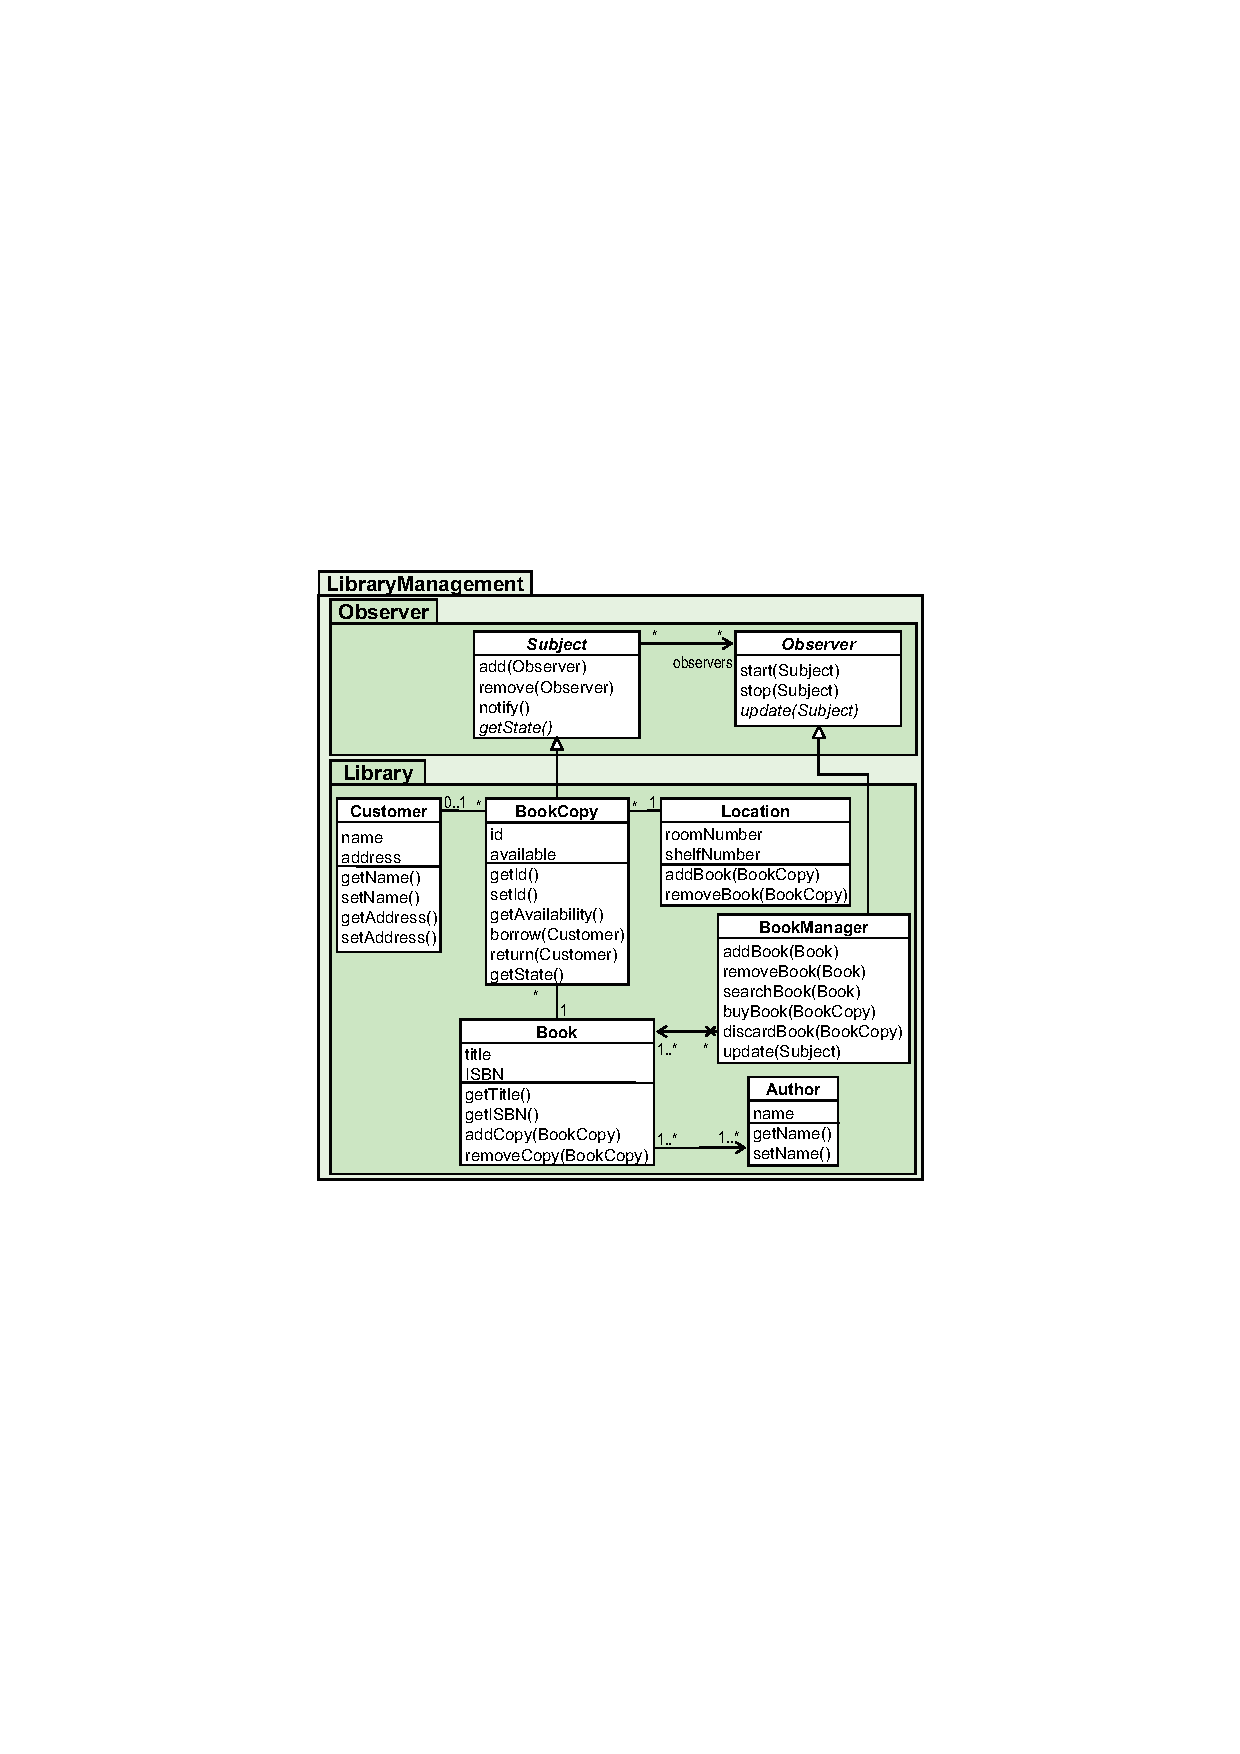
\includegraphics[width=0.4\linewidth]{figures/figure1}
	\caption{xxx (Quelle zitieren, wenn nicht selbst erstellt)}
	\label{fig:xxx}
\end{figure}

%-----------------------------------------------------------------------
\subsection{Tabellen}
%-----------------------------------------------------------------------

Jede Tabelle muss im Fließtext referenziertw werden. Für Tabellen gelten die selben Regeln, wie für Abbildungen (siehe dazu Abschnitt \ref{sec:abbildungen}).

Eine Beispiel einer Tabelle ist in Tabelle \ref{tab:xxx} zu finden:
\begin{table}
	\centering
	\begin{tabular}{| >{\bfseries}l | c | r | }
		\hline
			\rowcolor{orange} \bfseries Linksbündig & \bfseries Zentriert & \bfseries Rechtsbündig \\
		\hline
		\hline
			Zeile 1 & xxx & xxx \\\hline
			Zeile 2 & xxx & \dots \\\hline
			\multirow{2}{*}{Zeile3}
			& xxx & xxx \\\cline{2-3}
			& xxx & xxx \\\hline
		\hline
			\multicolumn{3}{| c |}{xxx} \\\hline
	\end{tabular}
	\caption{xxx (Quelle angeben)}
	\label{tab:xxx}
\end{table}

Bitte beachten Sie, dass Tabellen generell so einfach wie möglich gehalten werden sollen. Tabelle \ref{tab:xxx} dient unter anderem dazu Studierenden zu zeigen, wie Tabellen in \LaTeX\xspace erstellt werden können und wie Farben verwendet werden.
%%%%%%%%%%%%%%%%%%%%%%%%%%%%%%%%%%%%%%%%%%%%%%%%%%%%%%%%%%%%%%%%%%%%%%%%
\chapter{Implementierung der Relay Attacke}
\label{sec:problemdescription}
%%%%%%%%%%%%%%%%%%%%%%%%%%%%%%%%%%%%%%%%%%%%%%%%%%%%%%%%%%%%%%%%%%%%%%%%

Ziel dieses Kapitels ist die Beschreibung der praktischen Durchführung der NFC Relay Attacke. Es soll gezeigt werden, dass es mithilfe weniger Modifikationen am Android Betriebssystem möglich ist, die NFC Signale eines POS Terminals an ein zweites mobiles Gerät weiterzuleiten und auf diesem eine mobile Zahlung zu initiieren. Es wird dargestellt, auf welche Art und Weise ein Eingreifen in die Kommunikation der Zahlungsanwendung mit der NFC Schnittstelle möglich ist und wie die Antwortsignale der Zahlung an das weit entfernte POS Terminal zurückgesendet werden können. 

Ebenfalls soll diskutiert werden, welche unterschiedlichen Komponenten zum Aufbau und zur Durchführung der Relay Attacke notwendig sind, wie diese implementiert wurden und welche Rolle sie bei der Durchführung der Attacke einnehmen. Auftretende Schwierigkeiten sowie getroffene Entscheidungen sollen ebenfalls dargelegt werden.

Am Ende dieses Kapitels soll eine funktionsfähige Proof-of-Concept Implementierung der Relay Attacke stehen, deren Umsetzung mit einfachen Methoden des Android Frameworks realisiert wird und die als Grundlage für weiterführende Forschungen dienen soll. 

\section{Aufbau der Implementierung}

Zur Durchführung der Attacke wurden zwei handelsübliche, NFC-fähige Android Smartphones für die Rolle des Angreifers sowie des Opfers verwendet. Auf dem Angreifer-Gerät, einem HTC U11, war hierbei die Android Version 8.0.0 (API 26) vorhanden, auf dem Opfer-Gerät, einem Google Nexus 5X wurde eine modifizierte Version des Android Open Source Projektes mit der Version \textbf{XXX} installiert. Welche Modifikationen an diesem Betriebssystem vorgenommen wurden, wird in Kapitel \textbf{XXX} detailliert beschrieben.

Umgesetzt wurde die Relay Attacke durch die Entwicklung einer Proof-of-Concept Hostcard Emulation App, die eine handelsübliche mobile Payment Applikation wie beispielsweise Android Pay simulieren soll. Diese Anwendung wurde auf dem Opfer-Gerät installiert und als Ziel der Attacke sollte die HCE App zur Durchführung einer Zahlung und Weiterleitung der Daten an den Angreifer angeregt werden, ohne dass sich das Opfer in der Nähe eines POS Terminals befindet. Die Entwicklung der HCE App wird in Kapitel \textbf{XXX} dargelegt. 

Die Kommunikation der Geräte wurde durch eine weitere mobile Anwendung, welche unabhängig von der HCE Applikation operiert, realisiert. Diese existiert sowohl auf dem Angreifer- als auch auf dem Opfer-Gerät und sorgt für eine Verbindung zwischen den Kommunikationspartnern über ein Wireless Local Area Network (WLAN). 

Diese Anwendung kommuniziert darüber hinaus auch mit dem Android Betriebssystem und sorgt für die Ausführung der HCE App, sobald ein Signal vom Angreifer-Gerät empfangen wird. Darüber hinaus wird auch die Antwort der HCE App, die eigentlich an die NFC Schnittstelle gesendet wird, ebenfalls von der Kommunikationsanwendung abgefangen und an den Angreifer weitergeleitet. Mit welchen Mechanismen die unterschiedlichen Kommunikationswege umgesetzt wurden, wird in Kapitel \textbf{XXX} genauer ausgeführt. 

Zur erfolgreichen Durchführung der Attacke sind Modifikationen am Android Betriebssystem notwendig. Diese sorgen dafür, dass die entwickelten Anwendungen die passenden Signale erhalten, um korrekt operieren zu können. Bei der Durchführung der Attacke wird angenommen, dass eine modifizierte Version des Android Source Codes auf dem Opfergerät installiert werden kann.
Die genaue Durchführung der Änderungen am Android Betriebssystem wird in Kapitel \textbf{XXX} beschrieben. 

In folgender Abbildung ist eine Übersicht der Relay Attacke und der zur Durchführung entwickelten Komponenten gegeben. 

\begin{figure}
	\centering
	\caption{Übersicht der Relay Attacke}
\end{figure}

In Abbildung \textbf{XXX} ist in erster Linie ein POS Terminal sowie ein Angreifer- und ein Opfer-Gerät dargestellt. Bei Kontakt mit dem Angreifer initiiert das POS Terminal eine kontaktlose Zahlung über NFC. Die Apdus werden direkt in der Kommunikationsanwendung empfangen und über die WLAN Verbindung an das Opfer weitergeleitet. Die Kommunikationsanwendung, die auf dem Opfer-Gerät standardmäßig im Hintergrund aktiv ist, empfängt die Signale, woraufhin sie eine Kommunikation mit der auf dem Opfer vorhandenen HCE Applikation startet und eine mobile Zahlung in die Wege leitet. 
Bei der Durchführung der Zahlung werden von der Zahlungsapplikation Response Apdus an die NFC Schnittstelle des Gerätes gesendet, nachdem die HCE Anwendung davon ausgeht, durch NFC aufgerufen worden zu sein. 
Das modifizierte Betriebssystem leitet nun diese Antworten wieder an die Kommunikationsanwendung zurück, welche diese über WLAN wiederum dem Angreifer mitteilt. Vom Angreifer-Gerät werden die Apdus schlussendlich an das POS Terminal zurückgeleitet und die Relay Attacke wurde erfolgreich durchgeführt. 

In den nachfolgenden Kapiteln wird ausgeführt, wie die einzelnen Komponenten im Detail umgesetzt wurden, um die beschriebene Funktionalität bereitzustellen. 


In diesem Kapitel wird die eigentliche Problemlösung in einem oder mehreren Unterkapiteln ausgeführt. Die Strukturierung dieser Kapitel ist naturgemäß sehr stark von der konkre Aufgabenstellung abhängig. Der Name dieses Kapitels ist anzupassen, z.B. Umfeldbeschreibung -- Fallbeispiel \dots, konkreter schreiben je nach Art Diplomarbeit/Fragestellung.
\makeatletter\ifthesis@masterthesis
Nachfolgend einige Beispiele für unterschiedliche Arten von Diplomarbeiten.

Bei einer Software-Entwicklungsarbeit bieten sich folgende Unterkapitel an:
\begin{itemize}
	\item Im Kapitel \enquote{Design} sollte die konzeptionelle Lösung vorgestellt, diskutiert und begründet werden. Das Ergebnis dieses Kapitels könnte beispielsweise eine Protokoll-Architektur sein.
	\item Im Kapitel \enquote{Modelle} erfolgt üblicherweise das Feindesign. In diesem Kapitel könnten beispielsweise einzelne Protokolle bzw. Algorithmen aus der vorher definierten Protokoll-Architektur eingeführt und diskutiert werden. Achtung: Generell darauf achten, bei der eingangs erläuterten Notation zu bleiben und nicht Synonyme zu verwenden, verwirrt den Leser.
	\item Das Kapitel \enquote{Implementierung} sollte sich dann vorwiegend mit den Details der Umsetzung befassen. In diesem Kapitel sollte nur im Ausnahmefall exemplarisch Quellcode vorgesehen werden. Vielmehr sollten alle Probleme, die bei der Realisierung aufgetreten sind, dokumentiert, interpretiert und die Lösung erläutert werden.
\end{itemize}

Bei einer Arbeit zu einem abstrakteren Thema, bei dem ein oder mehrere Fallbeispiele aus der industriellen Praxis bearbeitet werden, bieten sich folgende Unterkapitel an:
\begin{itemize}
	\item Im Unterkapitel \enquote{Analyse der Problemstellung} wird die konkrete Problemstellung (die Situation im betrachteten Unternehmen) der Fallbeispiele beschrieben. Das Ergebnis dieses Kapitels könnte eine schematische Netzwerk- oder Applikationsarchitektur sein.
	\item Im Unterkapitel \enquote{Fallbeispiel} sollte sich (analog zur Implementierung in der Software-Entwicklung) mit den konkreten Details der Umsetzung befassen. Hier wird dargelegt, wie das zuvor identifizierte Lösungsschema konkret zur Anwendung gelangen kann bzw. welche Probleme während des Umsetzungsprojekts aufgetreten sind.
\end{itemize}

Bei einer Arbeit, deren Grundlage eine Auswahl eines Softwaresystems ist, bieten sich folgende Unterkapitel an:
\begin{itemize}
	\item IST-Analyse
	\item Hardware und Softwareausstattung
	\item Beschreibung der Geschäftsprozesse
	\item Schwachstellenanalyse des Unternehmens
	\item SOLL-Konzeption
	\item Auswahlverfahren möglicher verfügbarer Systeme -- Kriterienkatalog
	\item Einführung des neuen Systems
\end{itemize}

Bei einer Arbeit, deren Fokus auf der Durchführung und Auswertung von Fragebögen liegt, bieten sich folgende Unterkapitel an:
\begin{itemize}
	\item Im Kapitel \enquote{Problemstellung und Fragebogendesign} wird die fachliche Problemstellung detailliert erläutert und der Inhalt des Fragebogens in Bezug zur Problemstellung dargestellt.
	\item Im Kapitel \enquote{Befragungsmethode} werden die Untersuchungsobjekte (z.B. Praktische Ärzte), die Grundgesamtheit (Anzahl praktische Ärzte in Venezuela), Stichprobengesamtheit und das Verfahren zur Stichprobenziehung und das Erhebungsverfahren (Verteilung und Rücklauf der Fragebögen) beschrieben.
	\item Im Kapitel \enquote{Auswertungsmethode} werden die möglichen Auswertungsmethoden aufgelistet und ggf. begründet die ausgewählte Methode beschrieben.
	\item Im Kapitel \enquote{Befragungsdurchführung} wird die Untersuchungsdurchführung (z.B. Zeit, Ort der Befragung, Zeitraum der gesamten Befragung, besondere für das Untersuchungsergebnis oder zukünftige Forschungsarbeiten relevante Vorkommnisse etc.) dargestellt.
\end{itemize}

Hier intensive Rücksprache mit Ihren jeweiligen Fachbetreuern halten, mehrere Diplomarbeiten der Fakultät zu diesem Themenbereich durchsehen. Unabhängig vom Typ der Diplomarbeit werden im nachfolgenden Kapitel die konkreten Ergebnisse beschrieben.
\fi\makeatother
\chapter{Hinweise zur Literatur}
\label{sec:references}

\section{Literatursuche}

Der Vollzugang zu einigen Publikationen ist nur intern aus dem TU-Netz möglich. Um auf möglichst viele Papers extern zugreifen zu können, wird von der TU Wien eine \href{http://www.zid.tuwien.ac.at/tunet/vpn/extern/}{VPN-Zugangsmöglichkeit} angeboten, diesen VPN-Zugang bitte gleich einrichten.

Besonders ergiebig sind folgende Search-Engines:\\
\href{http://academic.research.microsoft.com/}{Microsoft Academic}\\
\href{http://dl.acm.org/}{ACM-Datenbank}\\
\href{http://scholar.google.com/}{Google Scholar}

Wir empfehlen, vor Beginn Ihrer Arbeit einige Diplomarbeiten, die am INSO oder generell an der Fakultät für Informatik verfaßt wurden, zu Ihrem Themenbereich zu suchen und Aufbau, Schreibstil, Art der Abbildungen etc. durchzuschauen. Arbeiten finden Sie \href{http://media.obvsg.at/tuw?query=grechenig&metaname=swishdefault&submit=Suche+starten&sbm=tuw*&lbm=*&lbc=*&searchtype=sim&.cgifields=metaname}{hier}.

Weitere Datenbanken und Suchmaschinen:\\
\href{http://rzblx1.uni-regensburg.de/ezeit/search.phtml?bibid=UBTUW&colors=7&lang=de}{Elektronische Zeitschriftenbibliothek der TU Wien}\\
\href{http://citeseer.ist.psu.edu/index;jsessionid=BF9BD5A89D42210F60E5CA88B40BAD9C}{Scientific Literature Digital Library (CiteSeer)}\\
\href{http://www.ingentaconnect.com/}{Ingenta}\\
\href{http://www.theiet.org/resources/inspec/}{INSPEC}

Journals:\\
\href{http://ieeexplore.ieee.org/}{IEEE - Institute of Electrical and Electronics Engineers, Inc. - Library}\\
\href{http://www.springerlink.com/?MUD=MP}{Verlag Springer - Springer Link}\\
\href{http://www.elsevier.com/wps/find/homepage.cws_home}{Elsevier}

Bibliotheken und Online-Kataloge:\\
\href{http://search.obvsg.at/primo_library/libweb/action/search.do?vid=ACC}{Online-Kataloge des Österreichischen Bibliothekenverbundes}\\
\href{http://aleph.ub.tuwien.ac.at/}{Online-Katalog der TU Wien} (ALEPH)\\
\href{http://www.informatik.uni-trier.de/}{Digital Bibliography \& Library Project (DBLP) of University of Trier}\\
\href{http://liinwww.ira.uka.de/bibliography/}{The Collection of Computer Science Bibliographies}

\section{BibLatex}

Biblatex bietet verschiedene Möglichkeiten an, um Literatur zu referenzieren. Die beiden häufigsten Befehle sind \verb|\cite| und \verb|\citeauthor|.

Beispiele wie referenziert werden kann:\\
\citeauthor{fankhauser:2009:softwaretechnik-security} beschreiben in \cite{fankhauser:2009:softwaretechnik-security} \dots\\
In \cite{schanes:2011:voip-fuzzer} zeigen \citeauthor{schanes:2011:voip-fuzzer} wie \dots
Weitere Informationen können in \cite{oasis:2010:homepage} von \citeauthor{oasis:2010:homepage} entnommen werden.

Wir empfehlen JabRef, um die Literaturdatenbank zu verwalten.

\chapter{Algorithmen und Quellcode}

\section{Beispiele für Quellcode}

Beispiel eines Quellcodes ist im Quellcode \ref{lst:shortcode} zu finden.

\begin{lstlisting}[caption={Short code},label=lst:shortcode]
//Start Program
System.out.println("Hello World!");
//End Program
\end{lstlisting}


\section{Beispiele für Algorithmen}

Algorithmus \ref{alg:samplealgorithm} dient als Beispiel.

\begin{algorithm}[t]
\SetKwData{Left}{left}
\SetKwData{This}{this}
\SetKwData{Up}{up}
\SetKwFunction{Union}{Union}
\SetKwFunction{FindCompress}{FindCompress}
\SetKwInOut{Input}{input}
\SetKwInOut{Output}{output}

\Input{A bitmap $Im$ of size $w\times l$}
\Output{A partition of the bitmap}

\BlankLine

\emph{special treatment of the first line}\;
\For{$i\leftarrow 2$ \KwTo $l$}{
\emph{special treatment of the first element of line $i$}\;
\For{$j\leftarrow 2$ \KwTo $w$}{\label{forins}
\Left$\leftarrow$ \FindCompress{$Im[i,j-1]$}\;
\Up$\leftarrow$ \FindCompress{$Im[i-1,]$}\;
\This$\leftarrow$ \FindCompress{$Im[i,j]$}\;
\If(\tcp*[r]{O(\Left,\This)==1}){\Left compatible with \This}{\label{lt}
\lIf{\Left $<$ \This}{\Union{\Left,\This}}\;
\lElse{\Union{\This,\Left}\;}
}
\If(\tcp*[r]{O(\Up,\This)==1}){\Up compatible with \This}{\label{ut}
\lIf{\Up $<$ \This}{\Union{\Up,\This}}\;
\tcp{\This is put under \Up to keep tree as flat as possible}\label{cmt}
\lElse{\Union{\This,\Up}}\tcp*[r]{\This linked to \Up}\label{lelse}
}
}
\lForEach{element $e$ of the line $i$}{\FindCompress{p}}
}
\caption{Sample algorithm}\label{alg:samplealgorithm}
\end{algorithm}

%%%%%%%%%%%%%%%%%%%%%%%%%%%%%%%%%%%%%%%%%%%%%%%%%%%%%%%%%%%%%%%%%%%%%%%%
\chapter{Analyse der Attacke}
\label{sec:results}
%%%%%%%%%%%%%%%%%%%%%%%%%%%%%%%%%%%%%%%%%%%%%%%%%%%%%%%%%%%%%%%%%%%%%%%%

Nach der erfolgreichen Durchführung der beschriebenen Relay Attacke, stellt sich die Frage, 
\section{Resultate}

\section{Anwendbarkeit}

\section{Folgen und Risiken}
Die Resultate der Arbeit präsentieren und nach Möglichkeit aussagekräftige, eigenständige Abbildungen einbauen. Namen des Kapitels konkretisieren, an jeweilige Arbeit anpassen -- Lösungsvorschlag/Implementierung im Titel des Kapitels benennen.
\makeatletter\ifthesis@masterthesis
Bei einer Soft\-ware-Ent\-wicklungs\-arbeit ggf. eine Beschreibung der Qualitätsmerkmale der neuen Implementierung (Performance, Sicherheit, Messergebnisse etc.) geben.

Bei einer Arbeit zu einem abstrakteren Architekturthema können hier die Eigenschaften nach der Anwendung der konzipierten Architektur beschrieben werden. Kommt sie in mehreren Fallbeispielen zum Einsatz, erfolgt hier ein Vergleich der jeweiligen Ergebnisse (z.B. gab es Unterschiede im Umsetzungserfolg, die sich auf konkrete Eigenschaften der betrachteten Fallbeispiele zurückführen lassen).

Bei einer Arbeit zur Softwareauswahl und Einführung wird eine Beschreibung von Qualitätseigenschaften des mit der Einführung neu geschaffenen SOLL-Zustands gegeben.

Bei einer Arbeit, deren Fokus auf der Durchführung und Auswertung von Fragebögen liegt, erfolgt in diesem Kapitel die Auswertung der Fragebögen.
\fi\makeatother
\makeatletter\ifthesis@masterthesis
%%%%%%%%%%%%%%%%%%%%%%%%%%%%%%%%%%%%%%%%%%%%%%%%%%%%%%%%%%%%%%%%%%%%%%%%
\chapter{Implementierung der Relay Attacke}
\label{sec:implementation}
%%%%%%%%%%%%%%%%%%%%%%%%%%%%%%%%%%%%%%%%%%%%%%%%%%%%%%%%%%%%%%%%%%%%%%%%

\section{ der Implementierung}

Zur Durchführung der NFC Relay Attacke wurden zwei handelsübliche, NFC-fähige Android Smartphones für die Rolle des Angreifers sowie des Opfers verwendet. Auf dem Angreifer-Gerät, einem HTC U11, war hierbei die Android Version 8.0.0 (API 26) vorhanden, auf dem Opfer-Gerät, einem Google Nexus 5X wurde eine modifizierte Version des Android Open Source Projektes mit der Version \textbf{XXX} installiert. Welche Modifikationen an diesem Betriebssystem vorgenommen wurden, wird in Kapitel \textbf{XXX} detailliert beschrieben.

Umgesetzt wurde die Relay Attacke durch die Entwicklung einer Proof-of-Concept Hostcard Emulation App, die eine handelsübliche mobile Payment Applikation wie beispielsweise Android Pay simulieren soll. Diese Anwendung wurde auf dem Opfer-Gerät installiert und als Ziel der Attacke sollte die HCE App zur Durchführung einer Zahlung und Weiterleitung der Daten an den Angreifer angeregt werden, ohne dass sich das Opfer in der Nähe eines POS Terminals befindet. Die Entwicklung der HCE App wird in Kapitel \textbf{XXX} dargelegt. 

Für die 

Die Kommunikation der Geräte wurde durch eine weitere mobile An
\fi\makeatother
%%%%%%%%%%%%%%%%%%%%%%%%%%%%%%%%%%%%%%%%%%%%%%%%%%%%%%%%%%%%%%%%%%%%%%%%
\chapter{Zusammenfassung und Ausblick}
\label{sec:conclusion}
%%%%%%%%%%%%%%%%%%%%%%%%%%%%%%%%%%%%%%%%%%%%%%%%%%%%%%%%%%%%%%%%%%%%%%%%

\makeatletter\ifthesis@masterthesis
Die Zusammenfassung ist nach der Kurzfassung der am häufigsten gelesene Teil, da viele Leser aus Zeitknappheit Arbeiten im Schnellverfahren konsumieren und rasch zur Zusammenfassung blättern. Hier hat man die Chance, dem Leser noch einmal die zentralen Ideen und Ergebnisse der Diplomarbeit zu vermitteln.

Im Gegensatz zur Kurzfassung sind die Leser mit der Problemstellung und der Terminologie bereits vertraut. In der Länge hat man deutlich mehr Spielraum als bei der Kurzfassung, die Zusammenfassung sollte inklusive Ausblick 2 bis max. 10 Seiten umfassen. Hier sollten kompakt die Antworten auf die in der Zielsetzung aufgeworfenen Fragen (Hypothesen) gegeben werden.

Neben einer Zusammenfassung der wichtigsten Ergebnisse sollte auch ein Ausblick gegeben werden: Aufzeigen des Bedarfs an zukünftiger Forschung, potentielle Anwendungsmöglichkeiten der vorgestellten Lösung etc.

In Summe sollte die Zusammenfassung dem Leser die wissenschaftliche und, wenn vorhanden, praktische Relevanz der Arbeit klar und verständlich darlegen.
\fi\makeatother

% insert bibliography and such stuff
\BackMatter

\cleardoublepage
\appendix

%%%%%%%%%%%%%%%%%%%%%%%%%%%%%%%%%%%%%%%%%%%%%%%%%%%%%%%%%%%%%%%%%%%%%%%%
\chapter{\appendixlabel}
%%%%%%%%%%%%%%%%%%%%%%%%%%%%%%%%%%%%%%%%%%%%%%%%%%%%%%%%%%%%%%%%%%%%%%%%

\whichlanguage{
Listings, data models, forms, \dots
}{
Quellcode, Datenmodell, Fragebögen, \dots
}

\end{document}
